\chapter [Plotting the Diode characteristics]{Plotting the Diode characteristics}


\section*{Problem definition}

This experiment requires to plot the forward characteristics of a diode. 

\section*{Background Details}
\paragraph{}

The charcteristic equation that governs the current flow throgh a diode when it is forward biased is given by:

\begin{equation}
Id=Is\ exp(\frac{Vd}{n Vt}-1)
\end{equation}
\paragraph{}

\section*{Let us experiment}

\paragraph{}
\begin{enumerate}
\item
Start Scilab on PC and Scilab console window opens. Create a new blank SciNote.
\item
The code for the required program is typed and saved as Scilab SCE file with an extension .sci
\item
The program is run using the “execute”.
\item
On executing the program in listing \ref{linEqn}, the following graph appears on the figure window

\end{enumerate}


\section*{SCILAB Code}
\subsection*{Plotting the diode characteristics}


\lstinputlisting[caption={Code to plot the voltage current graph of a diode},label={diodeFBchar}]{./scilabCode/diodeFBchar.sci}


\section*{Plot and Results}

For the program in listing \ref{diodeFBchar} the following figure \ref{diodeFBcharFig} results.

\begin{figure}
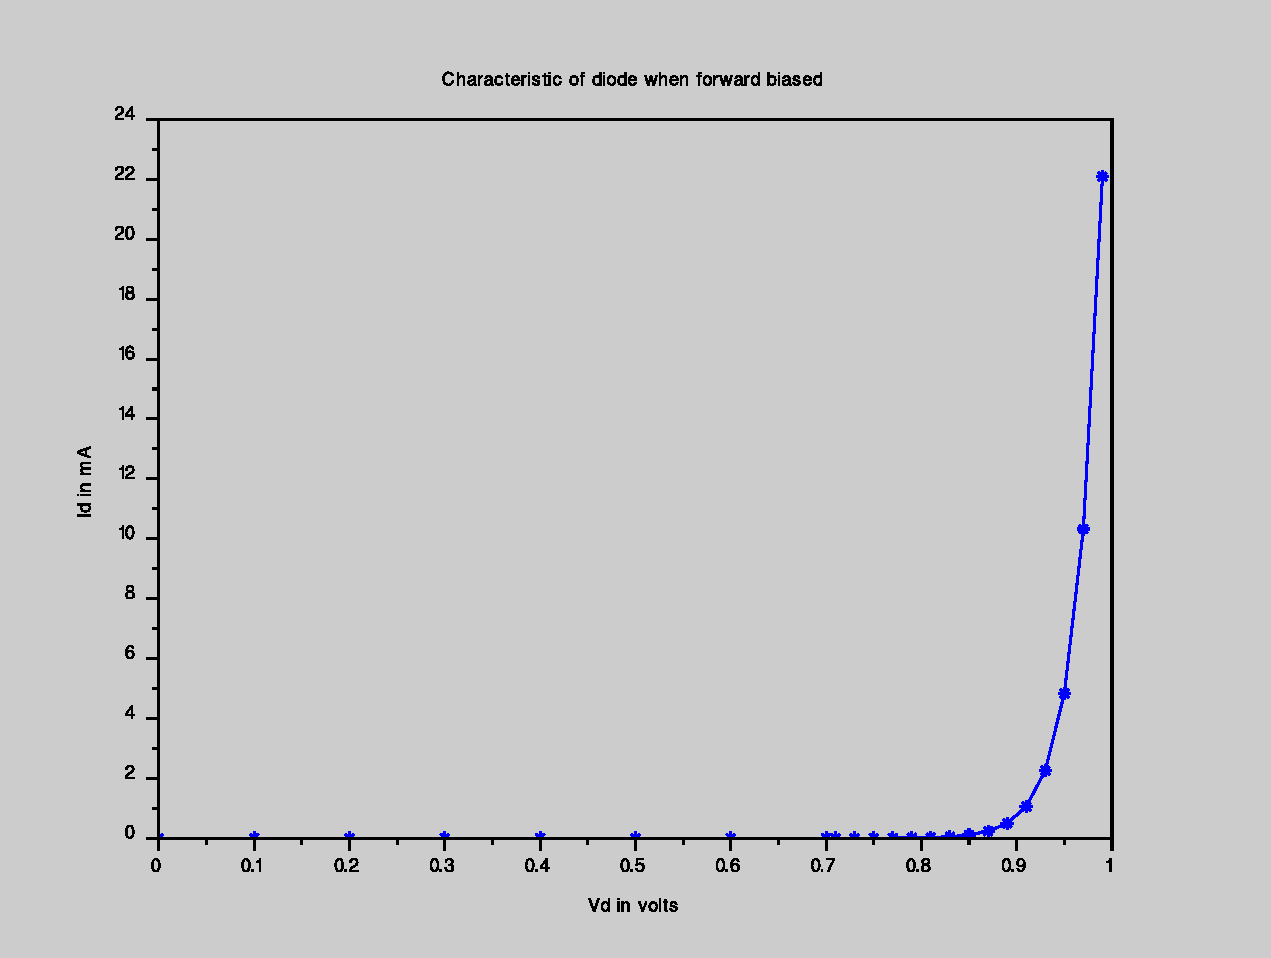
\includegraphics[width=\textwidth]{scilabCode/diodeFBchar.pdf}
\caption{Plot of Forward Characteristics of Diode}
\label{diodeFBcharFig}
\end{figure}
